\documentclass[11pt]{jarticle}
\usepackage{newcent}
\usepackage[dvipdfmx]{graphicx}
\usepackage{color}
\definecolor{purple}{rgb}{0.6,0,0.4}
\definecolor{brown}{cmyk}{0,0.81,1,0.60}
\definecolor{gray}{rgb}{0.4,0.4,0.4}
\definecolor{darkblue}{rgb}{0.0,0.0,0.6}
\definecolor{cyan}{rgb}{0.0,0.6,0.6}
\usepackage{listings,jlisting}
\renewcommand{\lstlistingname}{ソースコード}
\renewcommand{\slash}{/}
\lstdefinestyle{MyJava} % JavaとXML,2つの言語を使いたかったので.style=MyJavaとかで使い分け
{
language=Java, % lstlisting内の言語の指定
numbers=left, % 行番号を左端に表示する
breaklines = true, % 行が長くなってしまった場合の改行を行う
basicstyle={\small}, % 標準の書式設定
identifierstyle={\small}, % 識別子のスタイル
keywordstyle={\small\bfseries\color{purple}}, % キーワードのスタイル
commentstyle={\small\itshape\color{gray}}, % コメントのスタイル
stringstyle={\small\ttfamily\color{brown}}, % 文字列のスタイル
frame=single, % 枠のスタイル
tabsize=2, % タブ幅
showstringspaces=false, % 空白を可視化するか
}
\lstdefinelanguage{XML} % XMLはあまり充実してないってさー
{
    morestring=[b]",
    morestring=[s]{>}{<},
    morecomment=[s]{<?}{?>},
    stringstyle=\color{brown},
    identifierstyle=\color{darkblue},
    keywordstyle=\color{cyan},
    morekeywords={xmlns,version,type}% list your attributes here
}
\lstdefinestyle{MyXML} % JavaとXM(ry
{
language=XML,
numbers=left,
breaklines=true,
basicstyle={\small},
identifierstyle={\small\color{darkblue}},
keywordstyle={\small\bfseries\color{cyan}},
commentstyle={\small\itshape\color{gray}},
stringstyle={\small\ttfamily\color{brown}},
frame=single,
tabsize=2,
showstringspaces=false,
}
\usepackage{ascmac}
\usepackage{otf}
\usepackage[master]{gaiyo}

\title{スマートフォンのモーションセンサを利用した\\個人認証アプリケーションの開発に関する研究}
\id{15M7112}
\author{\UTF{9AD9}坂 賢佑}
\teacher{小林 孝史}

\begin{document}
\maketitle

% @suppress VoidSection
\chapter{序論}

% @suppress KatakanaSpellCheck
\section{研究背景}
% スマホ端末の急速な普及,それに伴う個人情報漏洩等のリスク
近年,スマートフォンと呼ばれる携帯端末が急速に普及しつつある.
スマートフォンとは,パーソナルコンピュータ向けに設計されたWebサイトを閲覧できる機能を持つフルブラウザを搭載し,様々な企業や個人が開発した多種多様なアプリケーションをインストールし利用できる携帯端末のことを指す\cite{1-smartphone}.
平成28年版の情報通信白書によるとスマートフォンの世帯普及率は2015年末時点で72.0\%とあり,また前年比で7.8ポイント増となっている\cite{1-spread}.
スマートフォンの普及によりどこでも手軽にオンラインショッピングやネットバンキングをはじめとする多種多様なサービスを利用できるようになった.

その一方で,これらサービスの利用にはユーザIDやパスワード等を含む個人情報を用いた個人認証を必要とする場合が多い.
また,利用しているブラウザやアプリケーションによっては,サービスにログインすれば一定期間ログイン状態を保持し再ログインの手間を省くような機能を持つものもある.
この機能により,ユーザはサービスを利用するたびに再ログインする手間が無くなることから利便性が向上する.
しかしながら,悪意のある第三者がサービスへのログインに必要な情報を知らずとも,本来のユーザになりすましてサービスを利用できてしまうという危険性がある.

% スマホ内の個人情報等を保護するための個人認証システムとその課題点
このように,スマートフォンは従来型のフィーチャーフォンと比較してより多くの個人情報を内包しており,第三者からのこれら情報への不正なアクセスを防ぐための仕組みが不可欠となっている.
現在この仕組みを実現する方法として広く採用されているのが,端末利用時にあらかじめ登録したパスコード情報や指紋情報をもとに,現在の利用者が本来の端末所有者であるかを確認する個人認証システムである.
パスコード認証方式では,あらかじめ端末所有者が特定の文字種からパスコードを構築し,これを端末に登録しておく.
そして,端末利用時に入力されたパスコードと登録されたパスコードを比較して同一であれば端末所有者であるとみなして,その後の端末利用を許可する.
指紋認証方式では,あらかじめ端末所有者が端末に搭載された指紋スキャナを通じて自らの指紋をスキャンし,これを端末に登録しておく.
そして,端末利用時に指紋をスキャンして登録された指紋との比較をし,同一であれば端末所有者であるとみなしてその後の端末利用を許可する.
これらの個人認証システムを利用することにより,第三者によって不正に端末内の個人情報へアクセスされる危険性をある程度軽減できる.
しかし,これらの認証方式にはそれぞれいくつかの問題点が挙げられる.

まずパスコード認証方式だが,これは個人認証を行う際にスマートフォン画面上に表示されたソフトウェアキーボードを目視し指でタッチして操作する必要があり,ユーザにとっては煩雑である可能性があるという点がある.
またあらかじめ決められた文字種の中から一つずつ選んだ文字を並べてパスコードを構築することから,パスコードのパターン数が限られ,認証に用いる鍵の自由度が制限されてしまうという点がある.

指紋認証方式については指紋をスキャンするためのハードウェアをスマートフォンに搭載しなければならないという点がある.
また指紋情報は変更ができないため,何らかの原因でこの情報が第三者に漏洩した場合は,今後その指紋を用いた個人認証ができなくなるという点がある.
さらに,ドイツのハッカー集団であるChaos Computer Clubの生体認証チームが,一般的なカメラで撮影された写真に写り込んだ指から指紋を複製することに成功している\cite{1-ccc}.
このことから,指紋情報が漏洩する可能性が十分にあり個人認証システムが担う機密性の確保が難しいといえる\cite{1-sophos}.

\section{研究目的}
% 前述した課題に対する本研究のアプローチ
本研究では,一般的なスマートフォンに搭載されている加速度センサと角速度センサを利用し,端末を振る動き(以下,モーション)で個人認証を行うシステムを開発する.
これによりパスコード認証方式における認証作業の煩雑さと鍵情報の自由度が制限されるという課題点を軽減し,指紋認証方式における指紋情報が漏洩した場合に鍵情報の変更ができないという課題点を解消した生体認証システムの実現を目指す.

\section{本論文の構成}
% 第2章以降の簡単な説明
第2章にて本研究に関連する先行研究について述べる.
第3章では本研究で開発した個人認証システムを提案するにあたり必要となる知識について説明する.
第4章では本研究で開発した個人認証システムの実装について,その詳細を述べる.
第5章では本研究で開発した個人認証システムの評価実験とその結果を示し,第6章で結論と今後の課題を述べたあと,本論文を総括する.

% @suppress JapaneseAmbiguousNounConjunction CommaNumber JapaneseNumberExpression
\section{システム概要}
本システムは,Android端末に一般的に搭載されている加速度センサと角速度センサを用いてモーションデータ(以下,データ)を収集し,人工ニューラルネットワークの一つであるDenoising Autoencoder(以下,dA)とその後ろに識別用ニューロンを繋げた識別器を用いて個人認証を行う.
%データの取得間隔はAndroid APIで用意された``SENSOR\_DELAY\_FASTEST''を指定しており,本システムの開発時に使用したNexus5ではおよそ5ミリ秒間隔でデータが取得できていることを確認した.
本システムではモーション入力を任意の時間で行えるが,データ数の差異を解決するため,登録モードでは入力時間の最も長かったものを,認証モードでは登録時に用いたものを基準にゼロによるパディングか末尾の切り落としを行う.
また,フーリエ変換を用いたローパスフィルタによりデータ入力時に生じる手の震えによる影響を減少させる.
さらに,加速度から変位,角速度から角度に変換したのち変位データを角度データで回転させ,データの変化が小さいことによる識別器の精度低下を防ぐために全データを1000倍したものを用いて以降の処理を行う.

登録モードでは,モーションの入力を任意回数で行える.
モーションが入力され前述のデータ加工をしたのち,CUDAサーバで動作するプログラム(以下,サーバ)にデータを送信する.
サーバでは,受信したデータについて平均が0,分散が1になるように正規化する.
そして,正規化したデータの30\%に平均が0で分散が1のガウシアンノイズによる加工を行う.
加工を行った後,dAの学習を行う.
学習データに加工を行ったデータを,教師信号に加工を行う前のデータを与え,損失関数に最小二乗誤差を用いて200回の学習を行う.
学習時のdAの構成は,中間層のニューロン数を入力層や出力層から30\%削減し,中間層の活性化関数にシグモイド関数,出力層の活性化関数に恒等関数を用い,中間層ニューロンのうち50\%をランダムにDropoutさせる.

dAの学習が終わればパラメータを固定して,その後ろに活性化関数にシグモイド関数を用いたニューロンを繋げる.
そして,データの20\%を0で上書きしたダミーデータを生成し,正規化する.
学習データに正規化したデータとダミーデータを,教師信号にそれぞれ0.0と1.0を与え,損失関数に交差エントロピー誤差を用いて誤差が0.1未満になるまで最大500回の学習を行う.
%この際Dropoutを無効にし,dAの出力に対して1から先ほどの学習時に適用したDropout率を引いた0.5を掛ける.
学習が終われば,識別器を構成するニューロンが持つパラメータを文字列として連結したデータを,クライアントに送信する.
クライアントは受信したパラメータを暗号化し,他アプリからの読み書きができない形で保存する.

認証モードでは,クライアントのモーション入力は1回のみ行える.
モーションが入力され前述のデータ加工をしたのち,サーバにデータと保存したパラメータを送信する.
サーバは,受信したデータを平均が0,分散が1になるように正規化する.
次に,受け取った学習済みニューラルネットワークのパラメータを元に識別器を構築する.
そしてこれに正規化したデータを与え,出力をクライアントに送信する.
クライアントはこれを受け取り,値が0.4未満であれば認証成功とし,0.4以上であれば認証失敗とする.
また,認証モードに限り,クライアントが何らかの理由でサーバに接続できない場合は,クライアント側でサーバと同様の処理を行うことができる.

\section{評価及び考察}
本システムの識別精度と登録及び認証処理にかかる時間を確認するため,実験を行った.
まず,端末を持ち上げるモーションを対象とした識別精度の評価実験を行った.
本システムを用いてあらかじめ6名の被験者にモーションを4回入力してもらい,モーションデータの収集を行った.
各被験者ごとに,最初の3回分を登録モードにおける訓練データとして用い,最後の1回分を認証モードにおける入力データとして10回認証を試行した.
また,それぞれの試行時になりすまし認証データとして筆者自身が同様のモーションを入力して得たモーションデータも入力した.
識別器より得られたデータを各被験者ごとに平均してまとめたものを表\ref{auth-result}に示す.

結果から,被験者Aと被験者B,被験者Fについては識別できているとわかる.
だが他の3名についてはなりすまし認証のモーションデータで得られた識別器の出力がより低く出ており,識別できていない.
本システムでは,端末所有者のモーションデータとなりすまし認証によるモーションデータを識別するためにダミーデータを用いた.
ダミーデータは元データの値域及び次元数に依存するため,これらが小さい場合は元データとの差があまり出ない可能性がある.
これにより,端末所有者が入力したモーションデータであってもなりすまし認証であると識別されてしまったのではないかと考えられる.
識別率の良かった被験者Aと良くなかった被験者Eのモーションデータを比較したものを図\ref{compare}に示す.

\begin{figure}[tbhp]
  \def\@captype{table}
  \begin{minipage}[t]{.48\textwidth}
    \centering
    \tblcaption{識別精度の評価結果}
    \label{auth-result}
    \begin{tabular}{|c|r||c|r|} \hline
      A & 0.091889 & なりすまし & 0.996035 \\ \hline
      B & 0.247552 & なりすまし & 0.492324 \\ \hline
      C & 0.098498 & なりすまし & 0.096458 \\ \hline
      D & 0.154409 & なりすまし & 0.123204 \\ \hline
      E & 0.637218 & なりすまし & 0.495835 \\ \hline
      F & 0.246713 & なりすまし & 0.32779536 \\ \hline
    \end{tabular}
  \end{minipage}
  %
  \hfill
  %
  \begin{minipage}[c]{.48\textwidth}
    \centering
    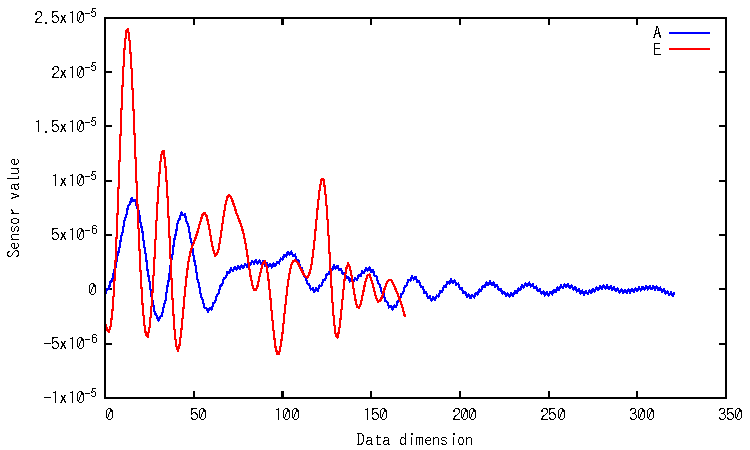
\includegraphics[bb=0 0 360 216, width=6cm]{Graphs/comp.pdf}
    \caption{被験者Aと被験者Eのモーションデータ比較}
    \label{compare}
  \end{minipage}
\end{figure}


次に,登録及び認証処理にかかる時間を計測するための実験を行った.

% @suppress JapaneseAmbiguousNounConjunction
\section{おわりに}
本研究では,Android端末に搭載されている加速度センサと角速度センサを用い,人間の動きで個人認証を行うシステムを開発した.
評価実験より,本人のモーション入力となりすましのモーション入力を上手く識別できた被験者が多かったものの,一部の被験者は識別できなかった.
本システムはダミーデータを作成して識別を試みたが,畳み込みニューラルネットワークのようなより高度な人工ニューラルネットワークを用いて,端末所有者の端末の振り癖を学習させることでより精度の高い個人識別が実現できる可能性があるため,引き続き研究を進めたい.

\end{document}
